\documentclass[acmcmpt, twoside]{acmsmall}

% Package to generate and customize Algorithm as per ACM style
\usepackage[ruled]{algorithm2e}
\renewcommand{\algorithmcfname}{ALGORITHM}
\SetAlFnt{\small}
\SetAlCapFnt{\small}
\SetAlCapNameFnt{\small}
\SetAlCapHSkip{0pt}
\IncMargin{-\parindent}

% Metadata Information
\acmVolume{1}
\acmNumber{1}
\acmArticle{1}
\acmYear{2012}
\acmMonth{4}

% Document starts
\begin{document}

% Page heads
\markboth{R. Yang \& Z. Jiang}{An Implementation of Surface Reconstruction from Point Set}

% Title portion
\title{An Implementation of Surface Reconstruction from Point Set}
\author{RUI YANG
\affil{Simon Fraser University}
ZHUOLI JIANG
\affil{Simon Fraser University}}

\begin{abstract}
Abstract goes here.
\end{abstract}

\keywords{MST, point set, PCA, Marching Cube}

\begin{bottomstuff}
Bottom stuff goes here.
\end{bottomstuff}

\maketitle

\section{Introduction}
In computing graphics, an important research area is the surface reconstruction from an unorganized 3D point set. The input point set has no connectivity, geometry and normal informations. Those points are on or near a surface $M$ that we want to derive a surface $M\prime$ to approximate. If we can recover the structure, topology and interconnectivity from an unknown point set, we can not only better understand the original characteristic of the point set and use the output for further processing, but also contribute solving this general problem that appears in other area such as MRI, laser range scanner, radar and seismic surveys and mathematical models. 
In early 90s, Hoppe et al[1] proposed an algorithm to infer the topology, the presence of boundaries and also geometry of surface $M$ from set of points $\{x_1,...,x_n\} \in R^3$. This algorithm is considered as a classic technique to solve surface reconstruction problem. Nowadays, several techniques are raised towards this problem or subset of this problem. For example, Poisson [2] is highly resilient to data noise but it assumes the orientation of points.   

\section{Algorithms}
Describe Input here. \\
What does each algorithms do \\
how these algorithms are connected. (What do they contribute to the whole implementation.)
\subsection{K Nearest Neighbours}

\subsection{Principle Component Analysis}
\subsection{K Euclidean Mininal Spanning Tree}
What is $k$-EMST, how it is different from normal EMST
\subsection{Normal Propagation}
\subsection{Marching Cubes}
Marching Cubes 
\begin{algorithm}[t]
\SetAlgoNoLine
\KwIn{Iso-level function, initial bounding cube, and maximum sub-divide level}
\KwOut{Result triangulated mesh}
$CubeStack$ = $\emptyset$; $Level$ = 0;
$Mesh$ = $\emptyset$\;
$InitialBoundingBox.Level$ = 0\;
$CubeStack$.push($InitialBoundingBox$)\;
\Repeat{$CubeStack$ is empty}{
	$CurrentCube$ = $CubeStack$.pop()\;
	
	Compute iso-level on each endpoints of $CurrentCube$\;
	\If{(iso-level on endpoints are all positive) \text{or}\\\ \ \ (iso-level on endpoints are all negative)}{
		Continue\;
	}
	\If{$CurrentCube$.$Level$ == $MaxLevel$}{
		Add proper triangle(s) to $Mesh$\;
	}\Else{
		\For{each one level smaller cube $SmallerCube$ in $CurrentCube$}{
			$CubeStack$.push($SmallerCube$);
		}
	}
}
\caption{Marching Cubes Algorithms}
\label{alg:mc}
\end{algorithm}

\section{Performance}
How our algorithms are doing.
\subsection{Output Quality}
\subsection{Time Complexity}
\subsection{Space Complexity}

\section{Discussion}
Why some of the output are bad, and why they cannot be solved for now.
\subsection{Variety of Input}
explain why horse.smf cannot be used as an input \\
how the result can be

\subsection{Iteration Methods of Marching Cubes}
divide and conquer vs. normal iteration (pros and cons) \\
explain possible holes in out implementation

\subsection{Size of Marching Cubes}

\section{Further Improvements}
What we have omitted. What can be done better
\subsection{Spacial Sensitive Structure}
How can our work be improved by using a better datastructure
\subsection{Refinement of Output Mesh}
The result mesh of our current implementation is composed of standalone triangles, i.e. Each vertex is included in only one triangle. This problem limits further processing of the output mesh. It can be solved by indexing all the vertices, and avoid generating a new vertex if one has existed at the same position.
\subsection{Cube Ambiguity Problem}



\cite{Lorensen-87}



\newpage
\newpage
\section{Introduction}

As a new technology, Wireless Sensor Networks (WSNs) has a wide
range of applications \cite{Culler-01,Bahl-02,Akyildiz-01}, including
environment monitoring, smart buildings, medical care, industrial and
military applications. Among them, a recent trend is to develop
commercial sensor networks that require pervasive sensing of both
environment and human beings, for example, assisted living
\cite{Akyildiz-02,Harvard-01,CROSSBOW} and smart homes
\cite{Harvard-01,Adya-01,CROSSBOW}.
% quote
\begin{quote}
``For these applications, sensor devices are incorporated into human
cloths \cite{Natarajan-01,Zhou-06,Bahl-02,Adya-01} for monitoring
health related information like EKG readings, fall detection, and voice recognition".
\end{quote}
While collecting all these multimedia information
\cite{Akyildiz-02} requires a high network throughput, off-the-shelf
sensor devices only provide very limited bandwidth in a single
channel: 19.2Kbps in MICA2 \cite{Bahl-02} and 250Kbps in MICAz.

In this article, we propose MMSN, abbreviation for Multifrequency
Media access control for wireless Sensor Networks. The main
contributions of this work can be summarized as follows.
% itemize
\begin{itemize}
\item To the best of our knowledge, the MMSN protocol is the first
multifrequency MAC protocol especially designed for WSNs, in which
each device is equipped with a single radio transceiver and
the MAC layer packet size is very small.
\item Instead of using pairwise RTS/CTS frequency negotiation
[\citeNP{Adya-01,Culler-01}; \citeNP{Tzamaloukas-01}; \citeNP{Zhou-06}],
we propose lightweight frequency assignments, which are good choices
for many deployed comparatively static WSNs.
\item We develop new toggle transmission and snooping techniques to
enable a single radio transceiver in a sensor device to achieve
scalable performance, avoiding the nonscalable ``one
control channel + multiple data channels'' design \cite{Natarajan-01}.
\end{itemize}

% Head 1
\section{MMSN Protocol}

% Head 2
\subsection{Frequency Assignment}

We propose a suboptimal distribution to be used by each node, which is
easy to compute and does not depend on the number of competing
nodes. A natural candidate is an increasing geometric sequence, in
which
% Numbered Equation
\begin{equation}
\label{eqn:01}
P(t)=\frac{b^{\frac{t+1}{T+1}}-b^{\frac{t}{T+1}}}{b-1},
\end{equation}
where $t=0,{\ldots}\,,T$, and $b$ is a number greater than $1$.

In our algorithm, we use the suboptimal approach for simplicity and
generality. We need to make the distribution of the selected back-off
time slice at each node conform to what is shown in Equation
(\ref{eqn:01}). It is implemented as follows: First, a random
variable $\alpha$ with a uniform distribution within the interval
$(0, 1)$ is generated on each node, then time slice $i$ is selected
according to the following equation:
% Unnumbered Equation
\[
i=\lfloor(T+1)\log_b[\alpha(b-1)+1]\rfloor.
\]
It can be easily proven that the distribution of $i$ conforms to Equation
(\ref{eqn:01}).

So protocols [\citeNP{Bahl-02,Culler-01,Zhou-06,Adya-01,Culler-01};
\citeNP{Tzamaloukas-01}; \citeNP{Akyildiz-01}] that use RTS/CTS
controls\footnote{RTS/CTS controls are required to be implemented by
802.11-compliant devices. They can be used as an optional mechanism
to avoid Hidden Terminal Problems in the 802.11 standard and
protocols based on those similar to \citeN{Akyildiz-01} and
\citeN{Adya-01}.} for frequency negotiation and reservation are not
suitable for WSN applications, even though they exhibit good
performance in general wireless ad hoc
networks.

% Head 3
\subsubsection{Exclusive Frequency Assignment}

In exclusive frequency assignment, nodes first exchange their IDs
among two communication hops so that each node knows its two-hop
neighbors' IDs. In the second broadcast, each node beacons all
neighbors' IDs it has collected during the first broadcast period.

% Head 4
\paragraph{Eavesdropping}

Even though the even selection scheme leads to even sharing of
available frequencies among any two-hop neighborhood, it involves a
number of two-hop broadcasts. To reduce the communication cost, we
propose a lightweight eavesdropping scheme.

\subsection{Basic Notations}

As Algorithm~\ref{alg:one} states, for each frequency
number, each node calculates a random number (${\textit{Rnd}}_{\alpha}$) for
itself and a random number (${\textit{Rnd}}_{\beta}$) for each of its two-hop
neighbors with the same pseudorandom number generator.
% Algorithm
\begin{algorithm}[t]
\SetAlgoNoLine
\KwIn{Node $\alpha$'s ID ($ID_{\alpha}$), and node $\alpha$'s
neighbors' IDs within two communication hops.}
\KwOut{The frequency number ($FreNum_{\alpha}$) node $\alpha$ gets assigned.}
$index$ = 0; $FreNum_{\alpha}$ = -1\;
\Repeat{$FreNum_{\alpha} > -1$}{
        $Rnd_{\alpha}$ = Random($ID_{\alpha}$, $index$)\;
        $Found$ = $TRUE$\;
        \For{each node $\beta$ in $\alpha$'s two communication hops
    }{
      $Rnd_{\beta}$ = Random($ID_{\beta}$, $index$)\;
      \If{($Rnd_{\alpha} < Rnd_{\beta}$) \text{or} ($Rnd_{\alpha}$ ==
          $Rnd_{\beta}$ \text{and} $ID_{\alpha} < ID_{\beta}$)\;
      }{
        $Found$ = $FALSE$; break\;
      }
        }
     \eIf{$Found$}{
           $FreNum_{\alpha}$ = $index$\;
         }{
           $index$ ++\;
     }
      }
\caption{Frequency Number Computation}
\label{alg:one}
\end{algorithm}

Bus masters are divided into two disjoint sets, $\mathcal{M}_{RT}$
and $\mathcal{M}_{NRT}$.
% description
\begin{description}
\item[RT Masters]
$\mathcal{M}_{RT}=\{ \vec{m}_{1},\dots,\vec{m}_{n}\}$ denotes the
$n$ RT masters issuing real-time constrained requests. To model the
current request issued by an $\vec{m}_{i}$ in $\mathcal{M}_{RT}$,
three parameters---the recurrence time $(r_i)$, the service cycle
$(c_i)$, and the relative deadline $(d_i)$---are used, with their
relationships.
\item[NRT Masters]
$\mathcal{M}_{NRT}=\{ \vec{m}_{n+1},\dots,\vec{m}_{n+m}\}$ is a set
of $m$ masters issuing nonreal-time constrained requests. In our
model, each $\vec{m}_{j}$ in $\mathcal{M}_{NRT}$ needs only one
parameter, the service cycle, to model the current request it
issues.
\end{description}

Here, a question may arise, since each node has a global ID. Why
don't we just map nodes' IDs within two hops into a group of
frequency numbers and assign those numbers to all nodes within two
hops?

\section{Simulator}
\label{sec:sim}

If the model checker requests successors of a state which are not
created yet, the state space uses the simulator to create the
successors on-the-fly. To create successor states the simulator
conducts the following steps.
% enumerate
\begin{enumerate}
\item Load state into microcontroller model.
\item Determine assignments needed for resolving nondeterminism.
\item For each assignment.
      \begin{enumerate}
      \item either call interrupt handler or simulate effect of next instruction, or
      \item evaluate truth values of atomic propositions.
      \end{enumerate}
\item Return resulting states.
\end{enumerate}
Figure~\ref{fig:one} shows a typical microcontroller C program that
controls an automotive power window lift. The program is one of the
programs used in the case study described in Section~\ref{sec:sim}.
At first sight, the programs looks like an ANSI~C program. It
contains function calls, assignments, if clauses, and while loops.
% Figure
\begin{figure}
% \centerline{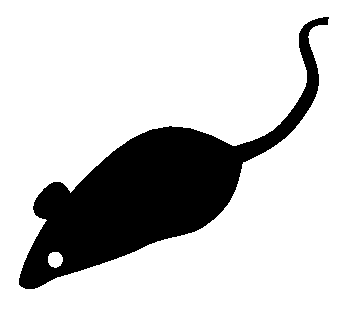
\includegraphics{acmsmall-mouse.eps}}
\caption{Code before preprocessing.}
\label{fig:one}
\end{figure}

\subsection{Problem Formulation}

The objective of variable coalescence-based offset assignment is to find
both the coalescence scheme and the MWPC on the coalesced graph. We start
with a few definitions and lemmas for variable coalescence.

% Enunciations
\begin{definition}[Coalesced Node (C-Node)]A C-node is a set of
live ranges (webs) in the AG or IG that are coalesced. Nodes within the same
C-node cannot interfere with each other on the IG. Before any coalescing is
done, each live range is a C-node by itself.
\end{definition}

\begin{definition}[C-AG (Coalesced Access Graph)]The C-AG is the access
graph after node coalescence, which is composed of all C-nodes and C-edges.
\end{definition}

\begin{lemma}
The C-MWPC problem is NP-complete.
\end{lemma}
\begin{proof} C-MWPC can be easily reduced to the MWPC problem assuming a
coalescence graph without any edge or a fully connected interference graph.
Therefore, each C-node is an uncoalesced live range after value separation
and C-PC is equivalent to PC. A fully connected interference graph is made
possible when all live ranges interfere with each other. Thus, the C-MWPC
problem is NP-complete.
\end{proof}

\begin{lemma}[Lemma Subhead]The solution to the C-MWPC problem is no
worse than the solution to the MWPC.
\end{lemma}
\begin{proof}
Simply, any solution to the MWPC is also a solution to the
C-MWPC. But some solutions to C-MWPC may not apply to the MWPC (if any
coalescing were made).
\end{proof}

\section{Performance Evaluation}

During all the experiments, the Geographic Forwarding (GF)
\cite{Akyildiz-01} routing protocol is used. GF exploits geographic
information of nodes and conducts local data-forwarding to achieve
end-to-end routing. Our simulation is
configured according to the settings in
Table~\ref{tab:one}. Each run lasts for 2 minutes and
repeated 100 times. For each data value we present in the results,
we also give its 90\% confidence interval.
% Table
\begin{table}%
\tbl{Simulation Configuration\label{tab:one}}{%
\begin{tabular}{|l|l|}
\hline
TERRAIN{$^a$}   & (200m$\times$200m) Square\\\hline
Node Number     & 289\\\hline
Node Placement  & Uniform\\\hline
Application     & Many-to-Many/Gossip CBR Streams\\\hline
Payload Size    & 32 bytes\\\hline
Routing Layer   & GF\\\hline
MAC Layer       & CSMA/MMSN\\\hline
Radio Layer     & RADIO-ACCNOISE\\\hline
Radio Bandwidth & 250Kbps\\\hline
Radio Range     & 20m--45m\\\hline
\end{tabular}}
\begin{tabnote}%
\Note{Source:}{This is a table
sourcenote. This is a table sourcenote. This is a table
sourcenote.}
\vskip2pt
\Note{Note:}{This is a table footnote.}
\tabnoteentry{$^a$}{This is a table footnote. This is a
table footnote. This is a table footnote.}
\end{tabnote}%
\end{table}%

\section{Conclusions}
Conclusions goes here.


% Bibliography
\bibliographystyle{acmsmall}
\bibliography{acmsmall-sam}

% History dates
%\received{February 2007}{March 2009}{June 2009}

\end{document}

